\documentclass{article}\usepackage[]{graphicx}\usepackage[]{color}
%% maxwidth is the original width if it is less than linewidth
%% otherwise use linewidth (to make sure the graphics do not exceed the margin)
\makeatletter
\def\maxwidth{ %
  \ifdim\Gin@nat@width>\linewidth
    \linewidth
  \else
    \Gin@nat@width
  \fi
}
\makeatother

\definecolor{fgcolor}{rgb}{0.345, 0.345, 0.345}
\newcommand{\hlnum}[1]{\textcolor[rgb]{0.686,0.059,0.569}{#1}}%
\newcommand{\hlstr}[1]{\textcolor[rgb]{0.192,0.494,0.8}{#1}}%
\newcommand{\hlcom}[1]{\textcolor[rgb]{0.678,0.584,0.686}{\textit{#1}}}%
\newcommand{\hlopt}[1]{\textcolor[rgb]{0,0,0}{#1}}%
\newcommand{\hlstd}[1]{\textcolor[rgb]{0.345,0.345,0.345}{#1}}%
\newcommand{\hlkwa}[1]{\textcolor[rgb]{0.161,0.373,0.58}{\textbf{#1}}}%
\newcommand{\hlkwb}[1]{\textcolor[rgb]{0.69,0.353,0.396}{#1}}%
\newcommand{\hlkwc}[1]{\textcolor[rgb]{0.333,0.667,0.333}{#1}}%
\newcommand{\hlkwd}[1]{\textcolor[rgb]{0.737,0.353,0.396}{\textbf{#1}}}%

\usepackage{framed}
\makeatletter
\newenvironment{kframe}{%
 \def\at@end@of@kframe{}%
 \ifinner\ifhmode%
  \def\at@end@of@kframe{\end{minipage}}%
  \begin{minipage}{\columnwidth}%
 \fi\fi%
 \def\FrameCommand##1{\hskip\@totalleftmargin \hskip-\fboxsep
 \colorbox{shadecolor}{##1}\hskip-\fboxsep
     % There is no \\@totalrightmargin, so:
     \hskip-\linewidth \hskip-\@totalleftmargin \hskip\columnwidth}%
 \MakeFramed {\advance\hsize-\width
   \@totalleftmargin\z@ \linewidth\hsize
   \@setminipage}}%
 {\par\unskip\endMakeFramed%
 \at@end@of@kframe}
\makeatother

\definecolor{shadecolor}{rgb}{.97, .97, .97}
\definecolor{messagecolor}{rgb}{0, 0, 0}
\definecolor{warningcolor}{rgb}{1, 0, 1}
\definecolor{errorcolor}{rgb}{1, 0, 0}
\newenvironment{knitrout}{}{} % an empty environment to be redefined in TeX

\usepackage{alltt}
\input{c:/aaaWork/zGnrlLatex/GnrlPreamble}
\hypersetup{pdftitle = R Workshop Install}
\input{c:/aaaWork/zGnrlLatex/JustRPreamble}
\setcounter{secnumdepth}{0}  % have unnumbered sections appear in TOC
\IfFileExists{upquote.sty}{\usepackage{upquote}}{}
\begin{document}


\section{Install R}
\begin{enumerate}
  \item Go to the RStudio CRAN\footnote{CRAN is an acronym for Comprehensive R Archive Network.} mirror (at \href{http://cran.rstudio.com/}{cran.rstudio.com}) in order to select the appropriate operating system for your computer\footnote{You can select a different mirror by going to \href{http://www.r-project.org/}{the R homepage}, selecting the ``download R'' link in the ``Getting Started'' box and selecting a mirror location from the ensuing page.}.  The remainder of these steps will illustrate the installation of R for the WINDOWS environment.
\begin{center}
  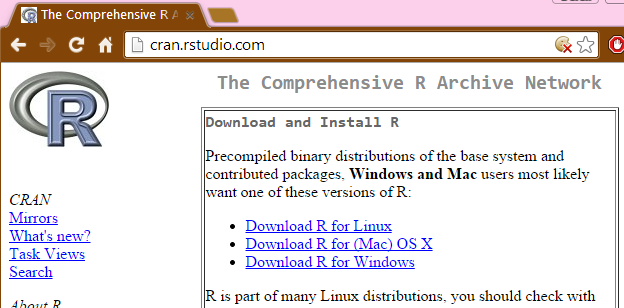
\includegraphics[width=4in]{Figs/R_Install_ChooseOS.png}
\end{center}

  \item Select the ``base'' option.
\begin{center}
  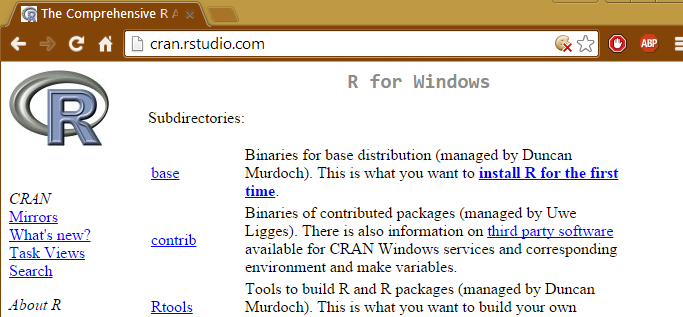
\includegraphics[width=4in]{Figs/R_Install_ChooseBase.png}
\end{center}

  \item Select the ``Download R 3.1.2 for Windows'' option (or similar if the version number has changed).  Make sure to note where you saved this executable program on your computer.
\begin{center}
  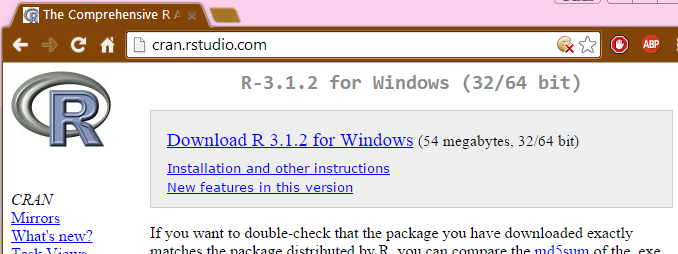
\includegraphics[width=4in]{Figs/R_Install_Download.png}
\end{center}

  \item Locate on your computer and run the downloaded file (called ``R-3.1.2-win.exe'' or similar if the version number has changed).  Select ``English'' language in the first dialog box (depending on your version of Windows you may have received security warnings before this dialog box appears).

  \item Press ``Next'' on the next two dialog boxes (the first is a simple description and the second is a user agreement).

  \item Select a location to install R (simply use the default location if the location is not important to you -- in the dialog box below I installed in a custom directory).  Press ``Next.''
\begin{center}
  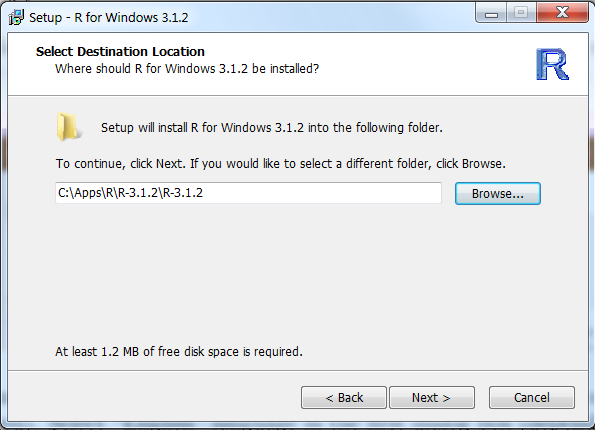
\includegraphics[width=2.5in]{Figs/R_Install_Directory.png}
\end{center}

  \item At this point you can choose to install 32- or 64-bit or both versions of R.  If you do not have a 64-bit computer, then you must install the 32-bit version.  If you do have a 64-bit computer, then I suggest, initially and for simplicity, installing only one version or the other.  I usually install the 32-bit version as it has some slight advantages when not working with extremely large data sets and with other software I have installed on my machine (see this \href{http://streaming.stat.iastate.edu/CRAN/bin/windows/base/rw-FAQ.html#Should-I-run-32_002dbit-or-64_002dbit-R_003f}{R FAQ}).  In this demonstration, I will install only the 32-bit version of R by de-selecting the ``64-bit Files'' option.  Press ``Next.''
\begin{center}
  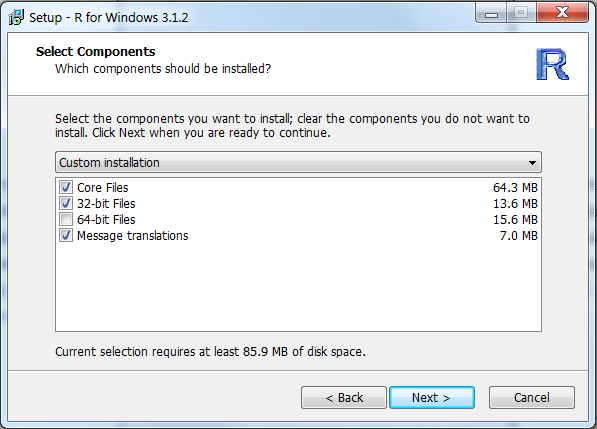
\includegraphics[width=2.5in]{Figs/R_Install_32Bit.png}
\end{center}

  \item Select the ``No (accept defaults)'' (this is the default) option.  Press ``Next.''

  \item Decide whether or not to create a shortcut in your Start Menu folder (I suggest that you do NOT).  Press ``Next.''

  \item Decide whether or not to create desktop or Quick Launch icons (top two choices) and whether to register the version number and associate .RData files with R (bottom two choices).  Generally, you will want to register the version number and associate the .RData files with R.  Press ``Next.''
\begin{center}
  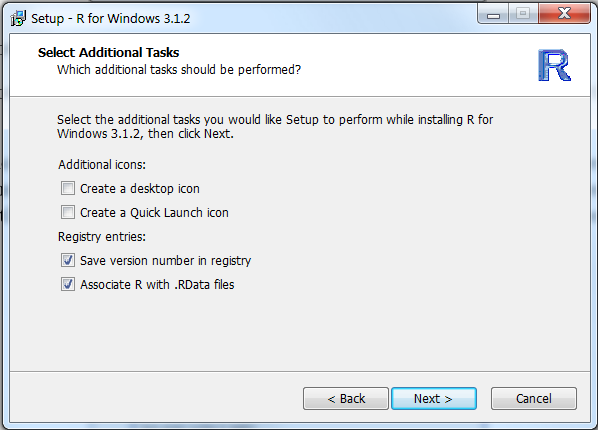
\includegraphics[width=2.5in]{Figs/R_Install_Options1.png}
\end{center}

  \item R should then begin installing files into the directory you chose previously.  If everything goes well, then you should get one last dialog box noting such.  Press ``Finish.''
%\begin{center}
%  \includegraphics[width=2.5in]{Figs/R_Install_Finish.png}
%\end{center}
\end{enumerate}


\section{Install RStudio}
\begin{enumerate}
  \item Go to the R Studio download page at \href{http://www.rstudio.com/products/rstudio/\#Desk}{www.rstudio.com/products/rstudio/\#Desk}.  Press the ``DOWNLOAD RSTUDIO DESKTOP'' button/graphic (near bottom-left).
\begin{center}
  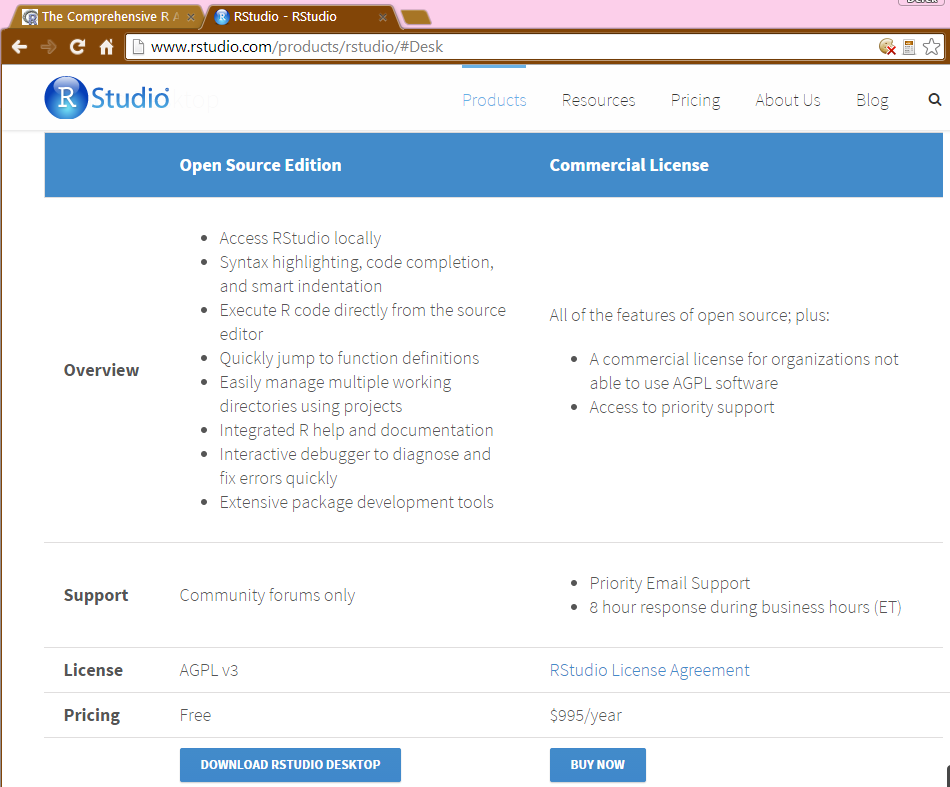
\includegraphics[width=4.9in]{Figs/RStudio_Install_Home.png}
\end{center}

  \item Select the link that corresponds to the operating system appropriate for your computer.  In the remainder of these directions I will demonstrate the installation for a WINDOWS operating system.  Make sure to note where this executable program is saved on your computer.
\begin{center}
  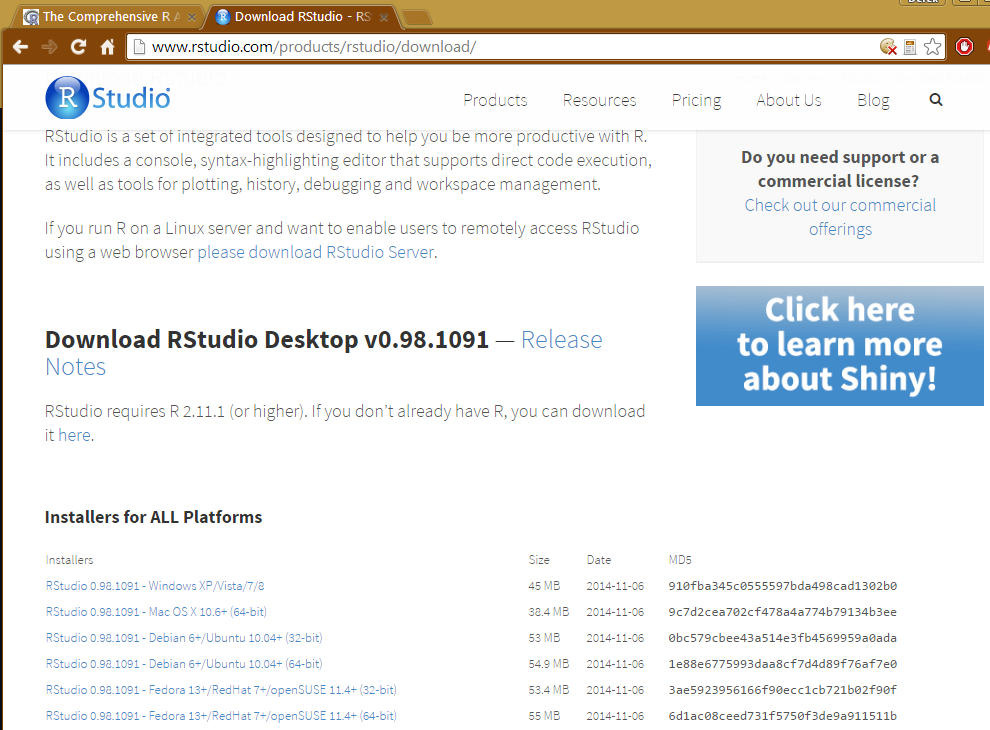
\includegraphics[width=4.9in]{Figs/RStudio_Install_ChooseOS.png}
\end{center}

  \item Locate and run the downloaded file (called ``RStudio-0.98.1091.exe'' or similar if the version number has changed).  Press ``Next'' on the first ``Welcome'' dialog box (depending on your version of Windows you may have received security warnings before this dialog box appears).

  \item Select a location to install RStudio (simply use the default location if the location is not important to you -- in the dialog box below I installed in a custom directory).  Press ``Next.''
\begin{center}
  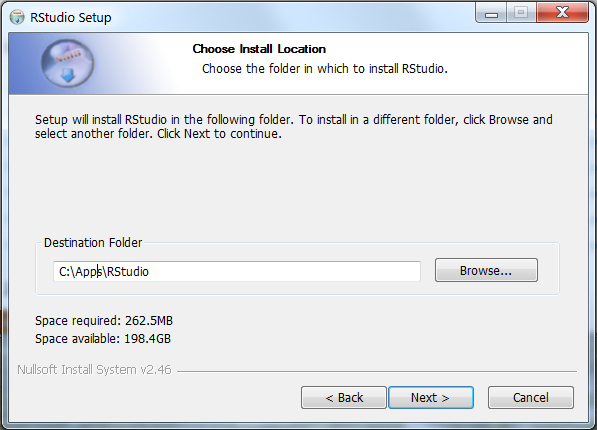
\includegraphics[width=2.5in]{Figs/RStudio_Install_Directory.png}
\end{center}

  \item Decide whether or not to create a shortcut in the Start Menu folder (I suggest that you do).  Press ``Install.''

  \item RStudio should then begin installing files into the directory you chose previously.  If everything goes well then you should get one last dialog box noting such.  Press ``Finish.''

  \item If you did not create a shortcut above then you will need to locate the ``rstudio.exe'' file inside the ``RStudio/bin'' folders inside the folder you chose to install RStudio in.  On my computer, for example this file is inside of ``C:/apps/RStudio/bin''.
\end{enumerate}

\end{document}
